% -----------------------------------------------
% Vlastní text práce (kapitoly práce)
% -----------------------------------------------

% -----------------------------------------------
\chapter{Calibration data analysis}
% -----------------------------------------------
In this section we present the analysis of calibration data, which we acquired by illuminating one FAST telescope (Argentina) by the older version of homogeneous UV LED source mounted into the IS. The older version of UV source was incapable of generating exact square pulse, and thus its output is deformed. However, the pulse's shape is stable and thus it was possible to use it for this experiment.   

\par
The main goal of this experiment is to obtain the relative responsivity ration constants for every of the four FASTs' PMTs (pixels) with respect to the pixel with greatest response for three positions of illumination - from left, right and bottom. Full specifications of the pixels numbering and positions could be seen on fig. \ref{PMT orientation}.

\begin{figure}[H]
 \centering
 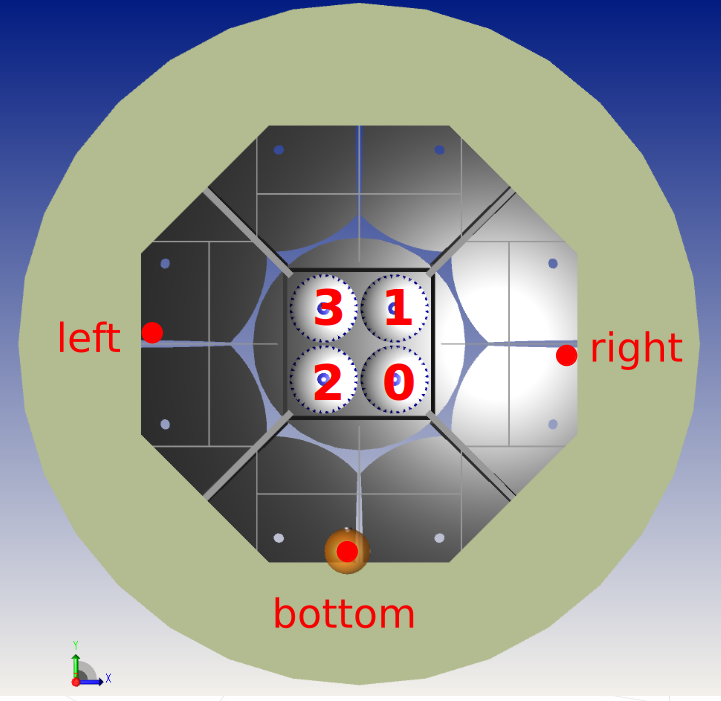
\includegraphics[scale=0.35, angle = 0]{./pictures/orientation2.png}
 \caption{Orientation of FASTs' PMTs (pixels).}
 \label{PMT orientation}
 
\end{figure}

\begin{figure}[H]
 \centering
 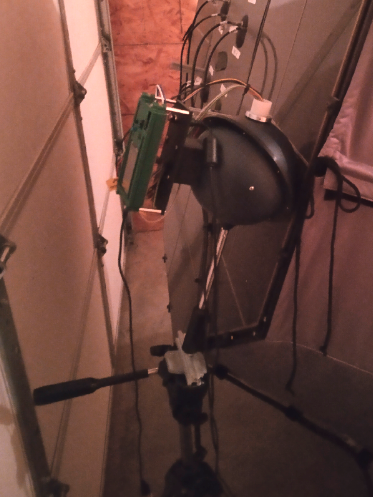
\includegraphics[scale=0.35, angle = 0]{./pictures/CalibMech.png}
 \caption{UV LED source mounted onto telescope.}
 \label{bottomCal}
 
\end{figure}
% -----------------------------------------------
\section{Calibration process}
% -----------------------------------------------
The UV source was mounted onto three positions and used as EULS to generate $8$ $\mu$s pulses. Two LED current levels were tested - $I_{d1} = 0.3$ mA and $I_{d2} = 0.8$ mA. These pulses trigger an event for the telescope - it acquires waveform data from every of the four PMTs. The PMTs' signal is converted into the number of photoelectrons registered in 20 ns. The example of detected 0.3 mA pulse from bottom position can be seen on fig (\ref{03pulse}). The 0.8 mA pulse is on fig. (\ref{08pulse}).

\begin{figure}[H]
 \centering
 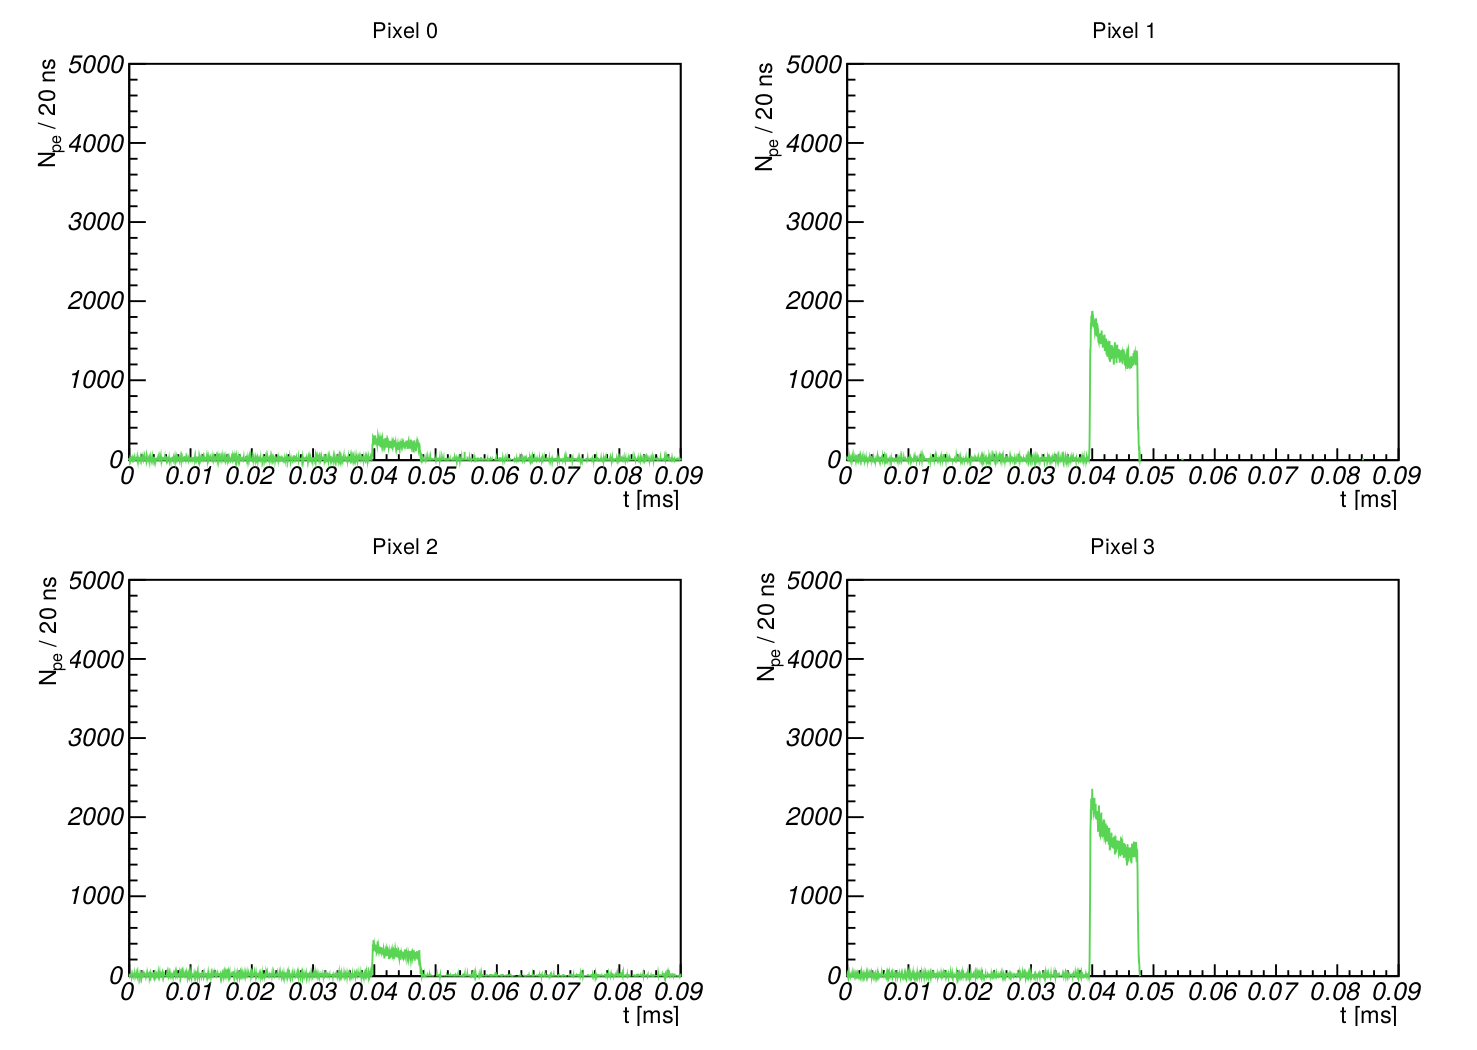
\includegraphics[scale=0.35, angle = 0]{./pictures/CalibPulses.png}
 \caption{0.3 mA pulse registered by all pixels.}
 \label{03pulse}
 
\end{figure}

\begin{figure}[H]
 \centering
 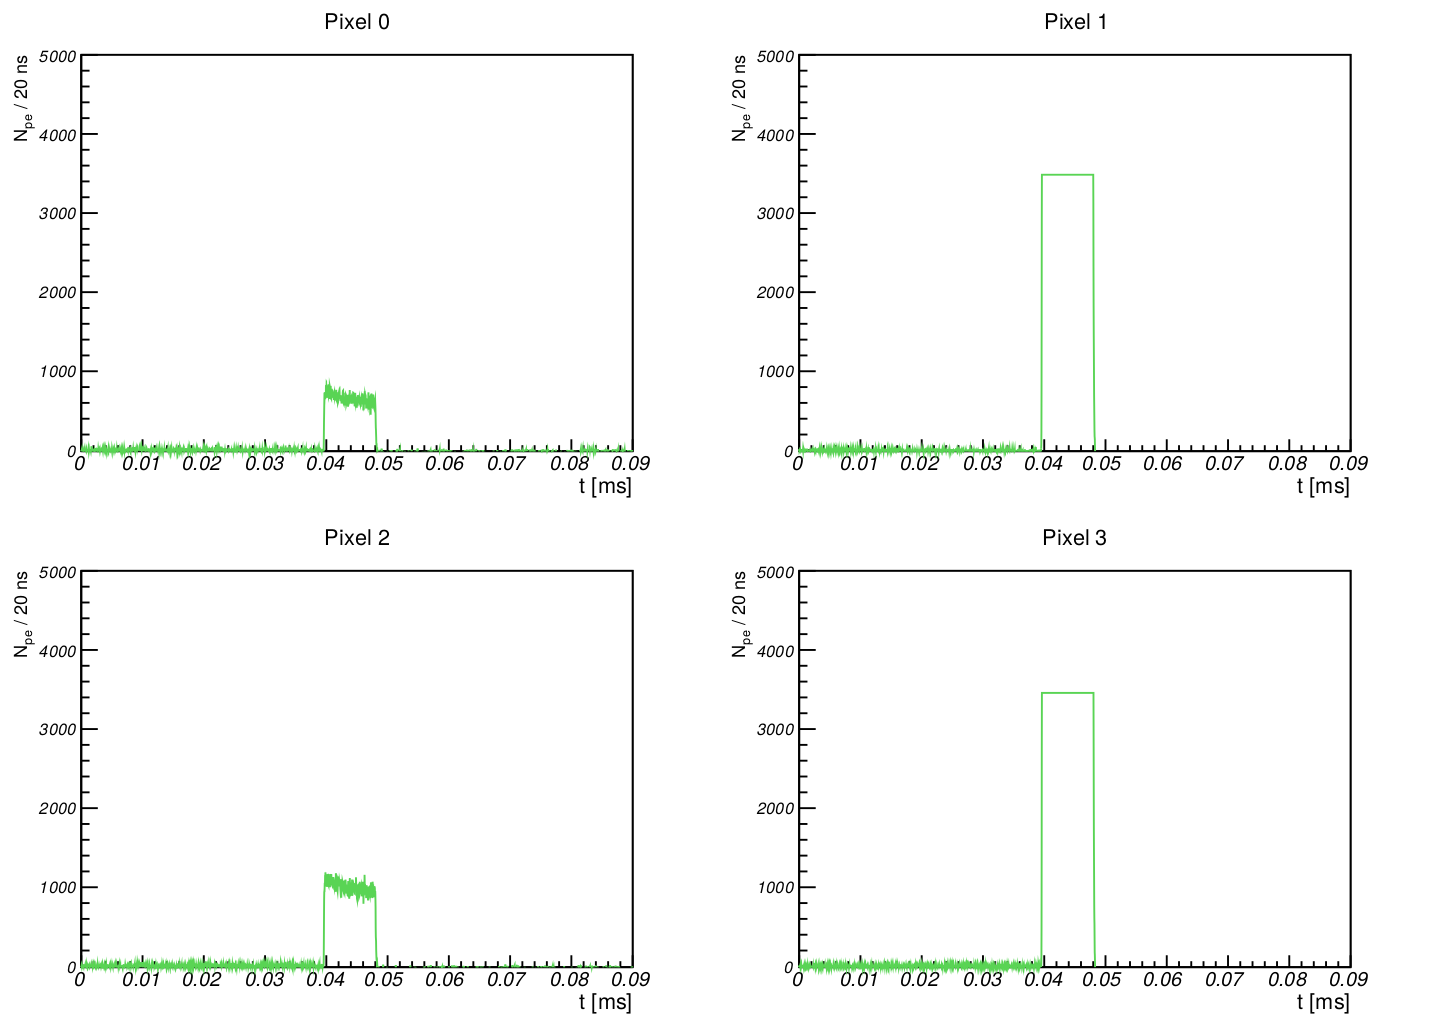
\includegraphics[scale=0.35, angle = 0]{./pictures/CalibSaturated.png}
 \caption{0.8 mA pulse saturated two pixels.}
 \label{08pulse}
 
\end{figure}


The fig. \ref{08pulse} shows that the 0.8 mA pulse saturated the pixel 1 and 3 and thus it is not possible to use them in analysis. 


\par
The 0.3 mA pulses are suitable for our analysis. However, due to their deformation we are not able to use analogous analysis scheme as we did for calibration source testing. The best parameter describing the collection efficiency of the PMT is the pulse's integral. 

% -----------------------------------------------

\section{Analysis and results}
% -----------------------------------------------
The data includes 4 waveforms for every detected pulse event and consists around 800 pulse events (for every position). From these signal waveforms we calculate the pulse's integral and then use these signal integrals to construct histograms. These histograms are fitted by gaussian. This process is repeated for all the three positions.
\par
The fitted histograms can be seen on fig. \ref{leftCal} (left), \ref{rightCal} (right) and \ref{bottomCal} (bottom).
\begin{figure}[H]
 \centering
 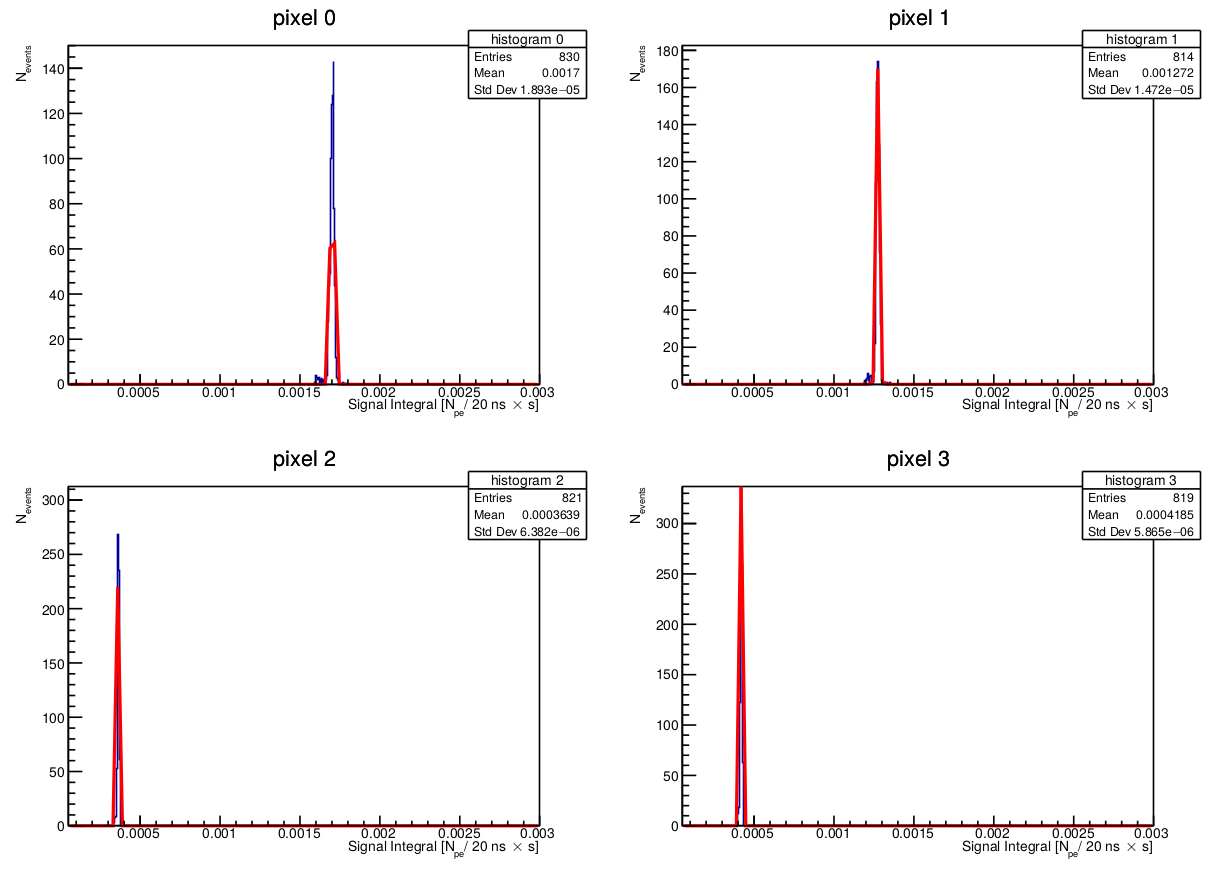
\includegraphics[scale=0.35, angle = 0]{./pictures/left.png}
 \caption{Signal integral histograms with gaussian fits for left position.}
 \label{leftCal}
 
\end{figure}
\begin{figure}[H]
 \centering
 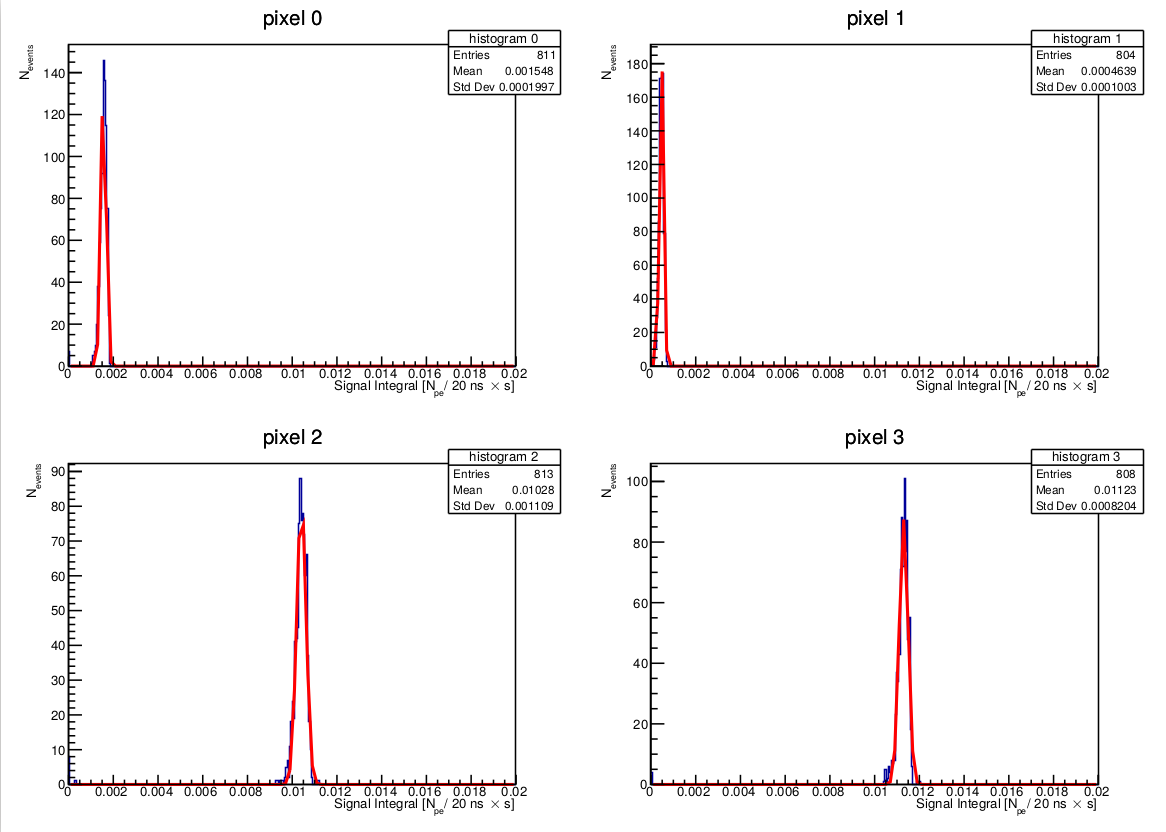
\includegraphics[scale=0.35, angle = 0]{./pictures/right.png}
 \caption{Signal integral histograms with gaussian fits for right position.}
 \label{rightCal}
 
\end{figure}
\begin{figure}[H]
 \centering
 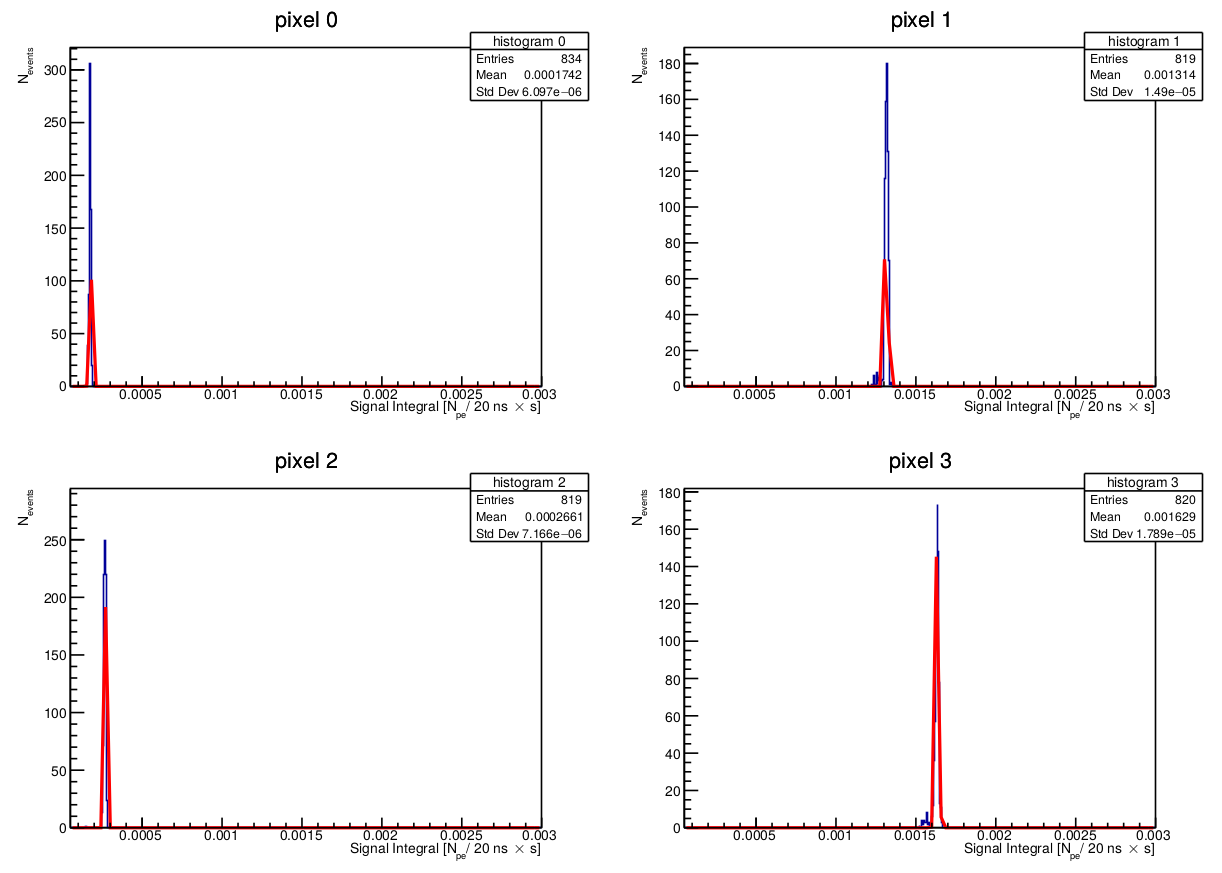
\includegraphics[scale=0.35, angle = 0]{./pictures/bottom.png}
 \caption{Signal integral histograms with gaussian fits for bottom position.}
 \label{bottomCal}
 
\end{figure}


The main parameter for determining responsivity ration constants is the mean value of the signal integrals, which is extracted from the gaussian. The relative calibration constants are calculated as follows:

\begin{equation}
c_{\textrm{i}} = \frac{m_{\textrm{i}}}{m_{\textrm{ref}}}.
\end{equation}

Where $c_{\textrm{i}}$ is a relative responsivity ration constants for i-th pixel, $m_{\textrm{i}}$ - associated mean value and $m_{\textrm{ref}}$ - mean value of the reference pixel. As the reference pixel is chosen the one with the greatest responsivity. 
\par
The associated error is:
\begin{equation}
\mu(c_{\textrm{i}}) = c_{\textrm{i}} \sqrt{(\frac{\mu(m_{\textrm{i}})}{m_{\textrm{i}}})^2 + (\frac{\mu(m_{\textrm{ref}})}{m_{\textrm{ref}}})^2}.
\end{equation}

As the basic errors $\mu(m_{\textrm{ref}})$ and $\mu(m_{\textrm{i}})$ are taken only the errors from the gaussian fits. Other systematic uncertainties were not yet determined and are not considered in this thesis.
\par
The results calculated by these equations for every position can be seen in the following table.

\begin{table}[H]
\centering
\begin{tabular}{|c|c|c|c|}
\hline
   & right & left & bottom \\ \hline
$c_0$ & $0.2314 \pm 0.0002$    & $1$   				   & $0.1070 \pm 0.0002$     \\ \hline
$c_1$ & $0.1397 \pm 0.0002$    & $0.7485 \pm 0.0003$   & $0.8061 \pm 0.0003$      \\ \hline
$c_2$ & $0.9304 \pm 0.0004$    & $0.2138 \pm 0.0002$   & $0.1631 \pm 0.0002$      \\ \hline
$c_3$ & $1$    				   & $0.2462 \pm 0.0002$   & $1$      \\ \hline
\end{tabular}
\caption{Table of calculated relative responsivity ration constants.}
 \label{CalibConstTbl}
\end{table}


%------------------------------------------------

\section{Simulation compartment and discussion}

To discuss the relevancy of measured and calculated values, we compare them to their counterparts from optical simulations, which were designed by Mgr. Martin Vacula from SLO. These simulations consists of theoretical models of FAST's mirrors and pixels illuminated by EULS in same three positions as was defined before. These models includes inhomogeneity correction matrixes for every pixel.

\begin{table}[H]
\centering
\begin{tabular}{|c|c|c|c|}
\hline
   & right & left & bottom \\ \hline
$c_0$ & $0.48$    & $0.95$   & $0.44$     \\ \hline
$c_1$ & $0.41$    & $1$   	 & $0.98$      \\ \hline
$c_2$ & $1$    	  & $0.41$   & $0.46$      \\ \hline
$c_3$ & $0.95$    & $0.46$   & $1$      \\ \hline
\end{tabular}
\caption{Table of simulated relative responsivity ration constants by Mgr. Martin Vacula.}
 \label{CalibConstTblSim}
\end{table}

The compartment between the two tables (theoretical simulation - \ref{CalibConstTblSim} and the real measurement - \ref{CalibConstTbl}) shows that the two pixels, which are lesser illuminated at the specified position have lesser responsivity than they should have according to the simulations.

\par
These differences may be caused by uncertainties in the EULS positioning, its partial space inhomogeneity, mirror inhomogeneity, or some yet undiscovered phenomena.


% -----------------------------------------------



% -----------------------------------------------
% %%%%%%%%%%%%%%%%%%%%%%%% End of file %%%%%%%%%%%%%%%%%%%%%%%%
